\documentclass[11pt]{article} 
%\documentclass[12pt]{article} 

\usepackage[utf8]{inputenc}
 
\usepackage[english]{babel}
\usepackage{lmodern}
\usepackage{setspace}
\usepackage{amsmath}

\usepackage[bottom]{footmisc}

\usepackage{parskip}
\setlength{\parindent}{20pt}
\setlength{\parskip}{1.3ex plus 0.5ex minus 0.3ex}

%% PAGE DIMENSIONS
\usepackage{geometry} % to change the page dimensions
\geometry{letterpaper} % or letterpaper (US) or a5paper 

%% GFX
\usepackage{graphicx} 
\DeclareGraphicsExtensions{.png,.jpg,.pdf}
\graphicspath{ {img/} }
\usepackage{float} 

%%% PACKAGES
\usepackage{booktabs} 
\usepackage{array} 
\usepackage{paralist}
\usepackage{verbatim}
\usepackage{subfig} 
\usepackage[xcdraw,dvipsnames]{xcolor}
% \usepackage[table,xcdraw,dvipsnames]{xcolor}

\usepackage{fancyvrb}
\usepackage{framed}
\usepackage{ellipsis}
\usepackage{csquotes}

%% If you use beamer only pass "xcolor=table" option, i.e. \documentclass[xcolor=table]{beamer}

%%% HEADERS & FOOTERS
\usepackage{fancyhdr} 
\pagestyle{fancy} 
\renewcommand{\headrulewidth}{0pt} 
\lhead{}\chead{}\rhead{}
\lfoot{}\cfoot{\thepage}\rfoot{}

%%% SECTION TITLE APPEARANCE
\usepackage{sectsty}
\allsectionsfont{\sffamily\mdseries\upshape}
% \subsectionfont{\sffamily\mdseries\upshape\noindent\fbox}
\subsectionfont{\sffamily\mdseries\upshape\noindent}

%%% ToC (table of contents) APPEARANCE
\usepackage[nottoc,notlof,notlot]{tocbibind}
\usepackage[titles,subfigure]{tocloft} 
\renewcommand{\cftsecfont}{\rmfamily\mdseries\upshape}
\renewcommand{\cftsecpagefont}{\rmfamily\mdseries\upshape} 

\usepackage[titletoc]{appendix}

%%% DEAD LAST
% \usepackage[colorlinks=true, linkcolor=teal, urlcolor=blue]{hyperref}
\usepackage[colorlinks=true, linkcolor=orange, urlcolor=blue]{hyperref}
\usepackage[english]{cleveref}
%% END Article customizations

%%% The "real" document content comes below...
\title{Sandow Plus Plus}
\author{Carlos Leyva Ayala (@Papitas at Nexus)}
\date{07/05/2020} 
\definecolor{shadecolor}{rgb}{0.92, 0.92, 0.92}

\newcommand{\bold}[1]{\textbf{#1}}
% \newcommand{\idea}[1]{ \colorbox{yellow!70}{#1} }
\newcommand{\idea}[1]{ \textcolor{red}{#1} }
\newcommand{\important}[1]{ \MakeUppercase{\bold{#1}} }
\newcommand{\code}[1]{\small\texttt{#1}}

\newcommand{\IFS}{\href{https://www.nexusmods.com/skyrimspecialedition/mods/25933}{IFS - Immersion-Friendly Sorting}}
\newcommand{\nbsp}{\hspace{2pt}}
\newcommand{\w}{Weight}
\newcommand{\W}{WGP}
\newcommand{\B}{Behavior}
\newcommand{\Bs}{Behaviors}


\newlength{\imgMed} 
\setlength{\imgMed}{10cm}

\newlength{\argdesc} 
\setlength{\argdesc}{10cm}


\begin{document}
\maketitle

\tableofcontents
\pagebreak

%%%%%%%%%%%%%%%%%%%%%%%%%%%%%
\section{Overview}
Thanks for using Sandow Plus Plus! \\
This mod is the result of many, MANY hours of hard work that sometimes required deep research\ldots and decompiling and trying to decipher how to use obscure  undocumented files that are already quite hard to come by per se.

\begin{figure}[H]
    \centering
    
\includegraphics[width=\imgMed]{flashback}
    \label{fig:flashback}
    \caption{The horror\ldots}
\end{figure}

The basic premise behind this mod is simple: \bold{train and sleep to gain \w{} and get muscular}\footnote{If you are playing as a woman and you gain boobs instead of muscles, you may want to try \href{https://www.nexusmods.com/skyrimspecialedition/mods/34593}{my favorite Bodyslide preset ever} (which I made myself, obviously).}. 

Nonetheless, this mod has become so complex\footnote{Don't worry, though. It has always been \bold{quite performant}} and has so many options it really deserves a full fledged help file.

%%%%%%%%%%%%%%%%%%%%%%%%%%%%%
\section{Really; read this document. I promise I tried my best not to be boring}
I always appreciate when authors take their time to explain how to use their mods and\ldots let us be honest: I hate when they don't bother to explain how to play their complex mods and such, so here we are.

So, let me emphasize again: \bold{Sandow Plus Plus is complex} and you should really read this document. \\
If you ever have a problem, I've most likely talked about it in this help file.

%%%%%%%%%%%%%%%%%%%%%%%%%%%%%
\section{Requirements}
Boring stuff, but necessary if you don't want me to ask you to enable debugging and tracing just for you to be greeted by a message telling you \href{https://knowyourmeme.com/memes/do-you-even-lift}{\important{Do you even read, bro?}}

\begin{figure}[H]
    \centering
    
\includegraphics[width=\imgMed]{brah}
    \label{fig:brah}
    \caption{Why, of course I'm not joking!}
\end{figure}

\pagebreak

%%%%%%%%%%%%%%%%%%%%%%%%%%%%%
\section{FAQ}
This section is actually composed of links to other parts of the document, and yes: I put it here on purpose because I know most of you won't bother to read the full guide\footnote{Your loss. You won't be able to bask in my sublime prose.}.

\subsection{My fatigue is over 9000!!!}
Dude\ldots you are an old meme and you were never funny to begin with.

\begin{figure}[H]
    \centering
    
\includegraphics[width=\imgMed]{9000}
    \label{fig:behavior-table}
\end{figure}

That being said, yes: that is expected if you don't sleep well. 

Remember Sandow Plus Plus is easygoing as long as you don't break its rules.

\subsection{Weight gaining for pure mages}
Yes. Brains and brawns have never been mutually exclusive in real life.
\begin{figure}[H]
    \centering
    
\includegraphics[width=\imgMed]{mishima}
    \label{fig:mishima}
\end{figure}

\subsection{What's the deal with the head resizing thing?}
Avoiding this:

\begin{figure}[H]
    \centering
    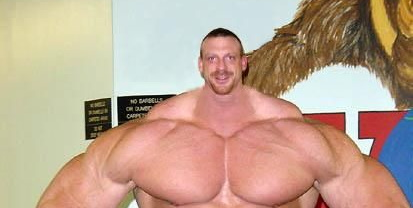
\includegraphics[width=\imgMed]{meme-head}
    \label{fig:meme-head}
\end{figure}

Also, opening the door to darkness.\\
I totally expect people\footnote{That could be even you!} asking me to make boobs and glutes bigger by using that marvelous technology.
\pagebreak

%%%%%%%%%%%%%%%%%%%%%%%%%%%%%
\section{The basics}
\begin{compactitem}
    \item  Every time a certain skill goes up, you get \code{Weight Gain Potential (\W)}, which transforms to \w{} when you sleep.
	\item So, train and sleep to gain \w.
\end{compactitem}

The basics are quite simple, so now let's talk about the complex stuff.

%%%%%%%%%%%%%%%%%%%%%%%%%%%%%
\section{\Bs}

\begin{figure}[h]
    \centering
    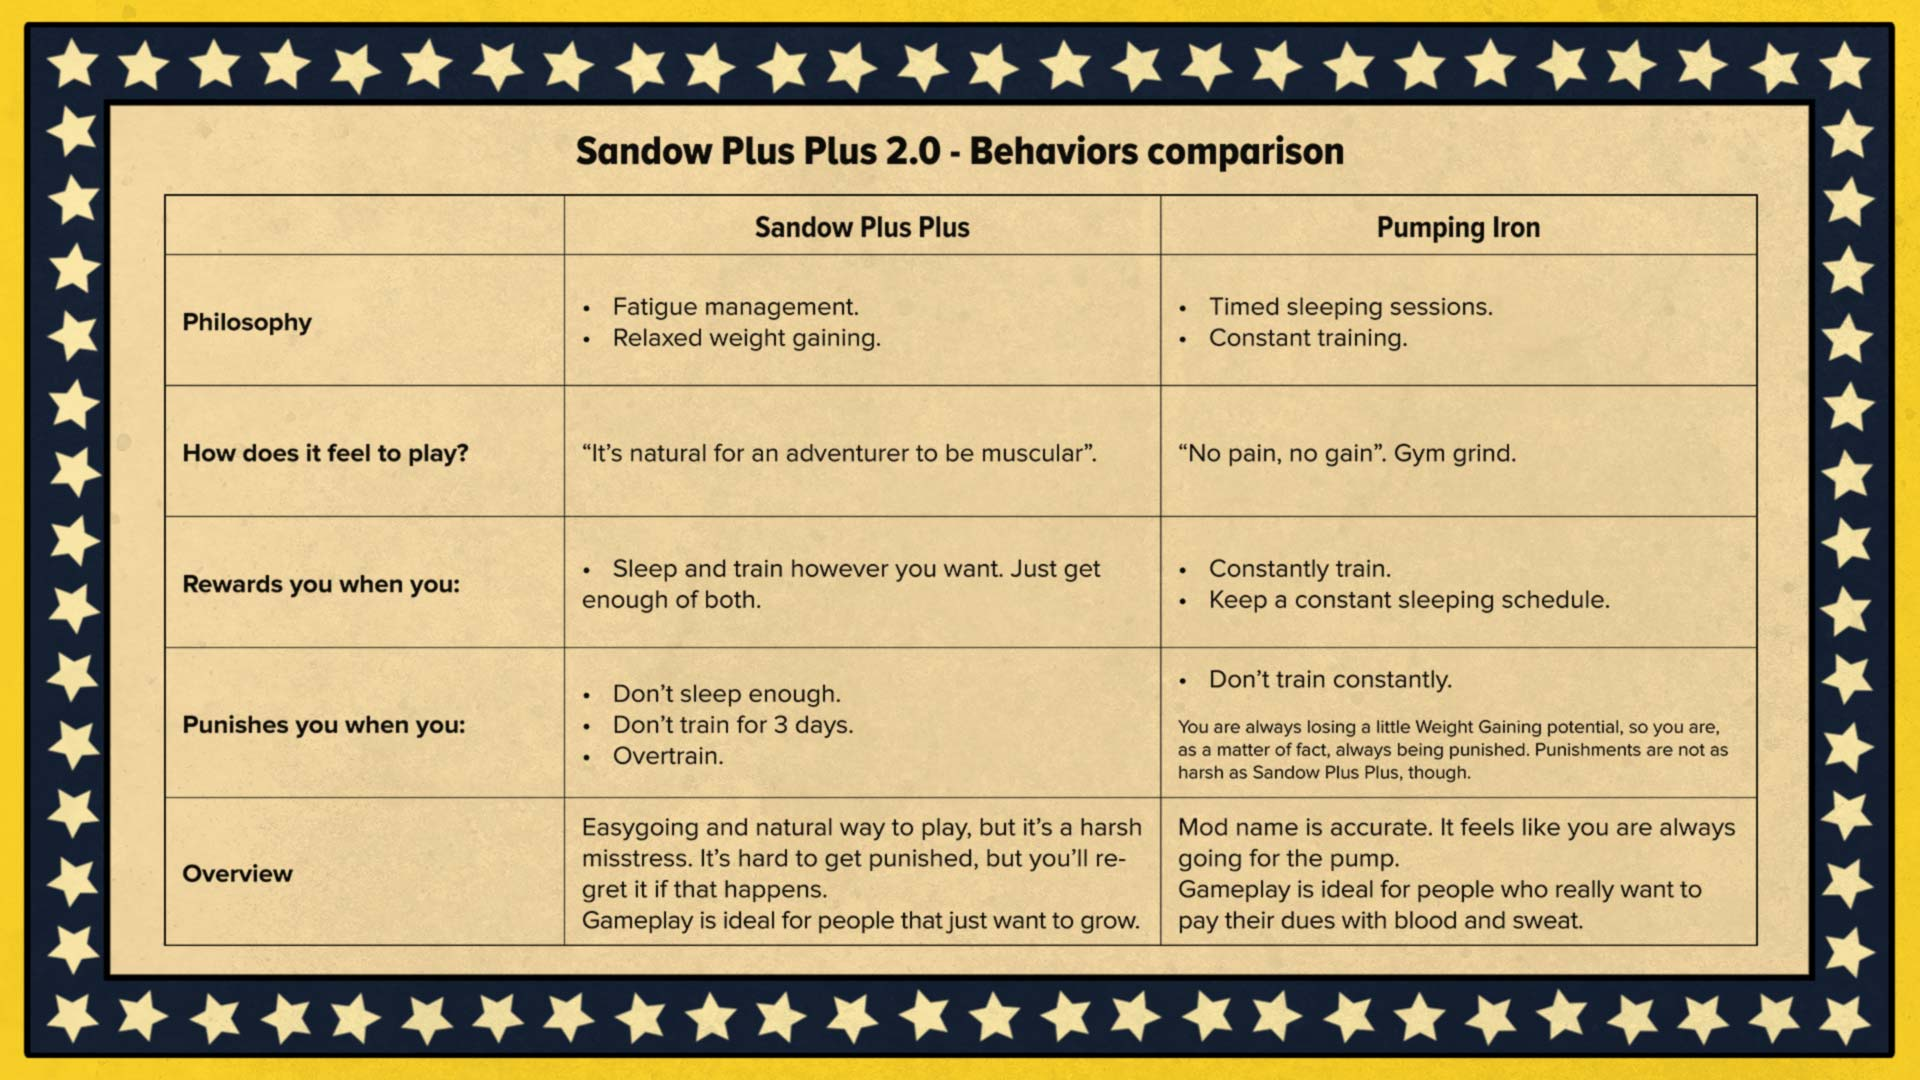
\includegraphics[width=\linewidth]{behavior-table}
    \caption{\Bs{} in v2.0}
    \label{fig:behavior-table}
\end{figure}

\Bs{} are rules to play this mod. The game feels quite different depending on which you choose.

To change \Bs, just select one from the MCM.

Let us start with the simplest and the one you are most likely accustomed to, since it's the most popular weight gaining mod in Skyrim.

%---------------------------------------------------------------
\section{The Pumping Iron \B}
When selecting this, you will get the exact same functionality you would expect from \href{https://www.nexusmods.com/skyrimspecialedition/mods/13434}{Pumping Iron}\footnote{Thanks to Gopher for graciously giving me permission for using his method!}, but you will also get all the \idea{quality of life additions native to this mod}.

\subsection{Summary}
\begin{table}[H]
    \centering
    \begin{tabular}{ll}
    \hline
     & \textbf{Summary} \\ \hline
    \textbf{Philosophy} & \begin{tabular}[c]{@{}l@{}}Timed sleeping sessions.\\ Constant training.\end{tabular} \\ \hline
    \textbf{How does it feel to play?} & “No pain, no gain”. Gym grind. \\ \hline
    \textbf{Rewards you when you:} & \begin{tabular}[c]{@{}l@{}}Constantly train.\\ Keep a constant sleeping schedule.\end{tabular} \\ \hline
    \textbf{Punishes you when you:} & \begin{tabular}[c]{@{}l@{}}Don’t train constantly.\\ You are always losing a little \W{},\\so you are, as a matter of fact, always being punished.\\Punishments are not as harsh as Sandow Plus Plus, though.\end{tabular} \\ \hline
    \textbf{Overview} & \begin{tabular}[c]{@{}l@{}}Mod name is accurate. It feels like you are always going \\for the pump.\\ Gameplay is ideal for people who really want to pay their \\dues with blood and sweat.\end{tabular} \\ \hline
    \end{tabular}
    \end{table}


\subsection{Mechanics}

Inactivity
You can lose weight by inactivity if the option to lose weight is checked. Right now that's the only way to lose weight using this behavior (you don't want more ways to lose weight; going from 0% to 100% is already quite hard).
The weight loss rate is 1% a day after 42 hours of not leveling up any skill that contributes to your WGP.

Be warned: those days are counted starting from the last time you trained. So if you haven't trained for 42 hours, you will lose 1.75% right off the bat.

Skill configuration
You can't configure your skill contribution to WGP because there's nothing stopping you from cranking everything up to max and make this a really boring mod (in the Sandow Plus Plus behavior doing that would lead to overtraining, but not here).
You will still get training from Sneak, Alteration and Restoration, though.

I'm quite aware mages will still get the short end of the stick.
I'll deal with that problem in a 'mmursive way in a future update.

Status reports
There's no fatigue in this behavior, so you get messages telling you how many hours you have left before you can sleep to gain weight, instead.
12 hours, as per Gopher design.


\begin{table}[]
    \centering
    \begin{tabular}{l|l}
    \hline
     & \textbf{Summary} \\ \hline
    \textbf{Philosophy} & \begin{tabular}[c]{@{}l@{}}Fatigue management.\\ Relaxed weight gaining.\end{tabular} \\ \hline
    \textbf{How does it feel to play?} & “It’s natural for an adventurer to be muscular”. \\ \hline
    \textbf{Rewards you when you:} & Sleep and train however you want. Just get enough of both. \\ \hline
    \textbf{Punishes you when you:} & \begin{tabular}[c]{@{}l@{}}Don’t sleep enough.\\ Don’t train for 3 days.\\ Overtrain.\end{tabular} \\ \hline
    \textbf{Overview} & \begin{tabular}[c]{@{}l@{}}Easygoing and natural way to play, but it’s a harsh misstress. \\ It’s hard to get punished, but you’ll regret it if that happens.\\ \\ Gameplay is ideal for people that just want to grow.\end{tabular} \\ \hline
    \end{tabular}
    \end{table}

Go around doing your own business to earn \W and just go to sleep when you are fatigued. That \W gets converted to weight if conditions are right.
% \item Gaining and losing weight is controlled by your fatigue. If you go to sleep with little fatigue, you'll only grow a little. Get too much fatigue and you'll start to lose WGP and maybe even weight!
% - Your gains can be affected by the law of diminishing returns: the more muscular you are, the harder is to get even more muscular (just like in real life). The opposite holds true. You can enable or disable this feature at will.
% - Sleep however you want; just get enough of it. No penalties for badly timed or short sleeping sessions.
% - Know your status without needing to open the MCM.
% - Right off the bat, Alteration and Restoration give you some WGP, but you can make other schools of magic give you some if that's what you want.
% - **Highly** configurable via MCM.
% - Save and load up to three different presets with your own configuration settings.
% - ESP flagged as ESL, so it only uses 1 slot out of 4096 instead of 1 out of 255. Save that precious space for bigger mods :)
% - From version 2.0 and on, you can play with all the rules of [Pumping Iron](https://www.nexusmods.com/skyrimspecialedition/mods/13434) but with all the QOL mechanics introduced by Sandow Plus Plus.



This mod is all about **fatigue managing**.
You'll only lose `WGP` if you go to sleep when your fatigue is above 90%. If your fatigue is 100% or above you'll also lose weight instead of gaining it (can be disabled in the MCM menu).

Weight gain is controlled by how much hours you sleep a day, but it's also controlled by fatigue. For best results, go to sleep 10 hours when you are somewhat fatigued (around 70% - 89.99%).
Sleeping more than 10 hours won't do anything for weight gaining, since your weight gain capabilities cap at 10 hours.
Of course, nothing stops you from sleeping 15 hours a day if it's more convenient to you. As I said, fatigue controls your gains, not time.

Always remember that **weight gaining depends on your WGP, how much you sleep and your fatigue**. You can certainly try to get cute and sleep 10 hours, wait 1 hour and then sleep again 10 hours, but you'll notice you won't gain as much as sleeping 10 straight hours when you are actually fatigued.

Fatigue builds two ways: over time and by leveling up skills.
Every single second awaken (in game time) you are getting fatigued. Also, each time you level up a skill that gives you WGP you get fatigued.
That means you'll get fatigued faster after a hard workout day compared to a shopping spree day.

And don't worry about performance. This mod only runs when you ask it to do it, and when it does, it's by performing simple mathematical formulas.

%%%%%%%%%%%%%%%%%%%%%%%%%%%%%
 

% \subsubsection*{Inputs}
% \begin{table}[H]
% \begin{tabular}{m{\argname} m{\argdesc}}
% \code{From} & ``What I don't want in the names?'' \\
% \code{To} & ``What I want instead.''
% \end{tabular}
% \end{table}

% %---------------------------------------------------------------
% \subsection*{Prepend}

% %---------------------------------------------------------------

% %---------------------------------------------------------------
% \subsection*{Trim front}
% Deletes blank spaces at the start of the name.

% %---------------------------------------------------------------
% \subsection*{Trim all}
% Deletes blank spaces both at the start and end of the name.

% %---------------------------------------------------------------
% \subsection*{Trim tail}
% Deletes blank spaces at the end of the name.

% %---------------------------------------------------------------
% \subsection*{Don't apply changes}
% When checked, the script will simulate the operations but not actually do them. Useful for watching what you will change before actually doing it. \\
% If you are satisfied with your results, run the script once again and uncheck this option.

% Enabled by default. \\
% If this feature annoys you, open the script, search for this line:


% \code{defaultDebugMode = true;}

% \noindent
% And change it to:

% \code{defaultDebugMode = false;}

% \noindent
% Now this feature is disabled by default.



% %%%%%%%%%%%%%%%%%%%%%%%%%%%%%
% \pagebreak
% \section{How to use -- Tutorial} \label{sec:tutorial}

% I wrote this tutorial so you can use my script in the way I designed it to work.\\
% In this tutorial, we are going from the simplest and most easy things, to more complex ones.

% I'm using the severely underrated sorting mod \IFS, so this tutorial will be written adhering to its author (astoundingly clever) conventions.

% Since this tutorial starts from the very beginning, if you already know how to create renaming mods you might want to skip that part and go directly to whatever function you would like to see in action. If so, use the table of contents to navigate as you please. 

% At any rate, even if you know what you are doing, I suggest you to start at the beginning of the tutorial at \cref{tut:prepend}, because it goes sequentially. 


% \begin{figure}[H]
%   \centering
%     \includegraphics[scale=1]{tut_fs000400_allDBcopied}
%   \caption{Your mod should look like this at this point}
%   \label{fig:tut_fs000400_allDBcopied}
% \end{figure}

% Right now you should have all armor, weapons and ingredients from Dragonbron copied to your mod, as you saw in \cref{fig:tut_fs000400_allDBcopied}.

% %||||||||||||||||||||||||||||||||||||||||||||||||||
% \begin{shaded}
% \begin{Verbatim}[fontsize=\scriptsize]
% ################ STARTING BATCH RENAMING (03:53:44 a. m.) ################
% Replacing "reagent" with "".

% "Reagent:Felsaad Tern Feathersreagent" renamed as "Reagent:Felsaad Tern Feathers"
% "Reagent:Emperor Parasol Mossreagent" renamed as "Reagent:Emperor Parasol Moss"
% "Reagent:Ash Creep Clusterreagent" renamed as "Reagent:Ash Creep Cluster"
% "Reagent:Netch Jellyreagent" renamed as "Reagent:Netch Jelly"
% "Reagent:Ash Hopper Jellyreagent" renamed as "Reagent:Ash Hopper Jelly"
% "Reagent:Boar Tuskreagent" renamed as "Reagent:Boar Tusk"
% "Reagent:Burnt Spriggan Woodreagent" renamed as "Reagent:Burnt Spriggan Wood"
% "Reagent:Spawn Ashreagent" renamed as "Reagent:Spawn Ash"
% "Reagent:Scathecrawreagent" renamed as "Reagent:Scathecraw"
% "Reagent:Trama Rootreagent" renamed as "Reagent:Trama Root"
% "Reagent:Ashen Grass Podreagent" renamed as "Reagent:Ashen Grass Pod"
% "Reagent:Hawk's Eggreagent" renamed as "Reagent:Hawk's Egg"
% "Reagent:Salmon Roereagent" renamed as "Reagent:Salmon Roe"
% "Reagent:Thorn Hookreagent" renamed as "Reagent:Thorn Hook"
% "Reagent:Screaming Mawreagent" renamed as "Reagent:Screaming Maw"
% "Reagent:Rot Scalereagent" renamed as "Reagent:Rot Scale"
% ################ ENDING BATCH RENAMING (03:53:44 a. m.) ################
% \end{Verbatim}
% \end{shaded}
% %||||||||||||||||||||||||||||||||||||||||||||||||||


% Thank you all for reading this and using my script. I see you all are people of culture as well.


\end{document}